\providecommand{\curso}{Primero Medio}
\providecommand{\colegio}{Colegio Divina Pastora}
\providecommand{\tituloDocumento}{Prueba 1}
\providecommand{\subtituloDocumento}{Homotecia y semejanza}

\documentclass{cdplf-prueba}

\begin{document}
%
\begin{tcbraster}[enhanced,raster columns=3,raster width=\linewidth,raster column skip=3pt,raster force size=false]
    \begin{caja}[title={\sffamily\scshape\bfseries Nombre},height=30pt,add to width=4cm]
    \end{caja}
    \begin{caja}[title={\sffamily\scshape\bfseries Puntaje},height=30pt,add to width=-2cm]
    \end{caja}
    \begin{caja}[title={\sffamily\scshape\bfseries Nota},height=30pt,add to width=-2cm]
    \end{caja}                    
\end{tcbraster}

\subsection*{Objetivos de la evaluación}
\begin{itemize}[]
    \item Aplican propiedades de la homotecia y semejanza para solucionar una \mbox{problemática}.
    \item Realizan homotecias en el plano cartesiano, conjeturan sobre el factor de la homotecia y las 
    \\\mbox{propiedades} de la imagen resultante.
    \item Explicar y fundamentar: 
    \begin{itemize}[]
        \item   Soluciones propias y los procedimientos utilizados.
        \item   Resultados mediante definiciones, axiomas, propiedades y teoremas.
    \end{itemize}
    %\item Explica soluciones propias y los procedimientos utilizados.
    %\item Elegir o elaborar representaciones de acuerdo a las necesidades de la actividad, identificando sus limitaciones y validez de éstas.
\end{itemize}

\subsection*{Instrucciones generales}

Esta evaluación, de cierre de unidad, abarca todos los contenidos trabajados en la unidad 
de geometría. Esta es individual, con nota al libro y no se puede usar calculadora para su 
desarrollo. 

\subsection*{Pauta de cotejo}

En la corrección de la evaluación, se le asignará puntaje a cada respuesta según
los criterios que se encuentran detallados en la tabla a continuación.

\begin{center}
    \begin{tblr}{width=\linewidth,colspec={X[1,c]|X[6]}, hline{1,Z} = {1}{-}{}, hline{1,Z} = {2}{-}{}, 
        hlines, cells={valign=m}, row{1} = {bg=black!15}}
        Puntaje asignado & \SetCell{c} Criterios o indicadores \\
        +50\% & Señala clara y correctamente cuál es la solución o el resultado de la pregunta hecha
        en el enunciado. \\ 
        +50\% & Incluye un desarrollo que relata de manera clara y ordenada los procedimientos 
         \mbox{necesarios} para solucionar la problemática. En caso de estar incompleto o con 
         \mbox{errores} el desarrollo, se asignará puntaje parcial si se muestra dominio de los 
         con\-tenidos y conceptos involucrados. \\
        0\% &  La respuesta es incorrecta. De haber desarrollo, este tiene errores conceptuales.\\
    \end{tblr}    
\end{center}
    
\vspace*{\fill}
\begin{center}
    \begin{tikzpicture}[ampersand replacement=\&,]
        %\node (A) [opacity=0.4] {\includegraphics[width=2cm]{../flork3.jpg}};
        \node (B) [font=\slshape,text width=12cm]
        {``Cree en ti mismo y en lo que eres. Sé consciente de que hay algo en tu interior %
        que es más grande que cualquier obstáculo''};
        \node [left=0mm of B,opacity=0.4] {\pgfornament[width=2cm]{37}};
        \node [right=0mm of B,opacity=0.4] {\pgfornament[width=2cm]{38}};
    \end{tikzpicture}
\end{center}
\vspace*{\fill}
\newpage

%\parte 
\begin{tcolorbox}[boxrule=1pt,colback=white,leftrule=3mm]
    \raggedright Resuelva los problemas que se encuentran a continuación. Para esto, no olvide 
    incluir un desarrollo pertinente y la respuesta al enunciado en los espacios señalizados.        
\end{tcolorbox}

\subsection{} Calcule el área [1 punto] y perimetro [4 puntos] del triángulo $ABC$.

\begin{center}
\begin{tikzpicture}[line width=1pt,scale=1.5]
    \draw (0,0) coordinate [label={[label distance=5pt]left:$A$}] (A) -- (30:3) %
        coordinate [label={[label distance=5pt,xshift=4pt]above:$C$}] (C) -- ([turn]-90:4) %
        coordinate [label={[label distance=5pt,yshift=-5pt]right:$B$}] (B) {} -- cycle;
    \draw (C) -- ($(A)!(C)!(B)$) coordinate (D);
    \draw (D) -- ($(C)!(D)!(B)$) coordinate (E);
    \draw (D) -- ($(D)!10pt!(A)$) -- ([turn]-90:10pt) -- ([turn]-90:10pt);
    \draw (E) -- ($(E)!10pt!(B)$) -- ([turn]-90:10pt) -- ([turn]-90:10pt);
    \draw (C) -- ($(C)!10pt!(A)$) -- ([turn]90:10pt) -- ([turn]90:10pt);
    \draw[decorate, decoration={calligraphic brace,raise=4pt,amplitude=10pt}]
        (C) -- (E) node [pos=0.5, right=15pt,yshift=10pt] {$\dfrac{36}{5}$};    
    \draw[decorate, decoration={calligraphic brace,raise=4pt,amplitude=10pt}]
        (E) -- (B) node [pos=0.5, right=15pt,yshift=10pt] {$\dfrac{64}{5}$};
\end{tikzpicture}
\end{center}

\begin{desarrollo}[height=10cm]
\end{desarrollo}
\begin{respuesta}[height=2cm]
\end{respuesta}

\subsection{} Aplique sobre la figura sombreada una homotecia con centro $O(13,4)$ y razón
$k = -0.5$. Dibuje la figura resultante en el plano [1 punto], y determine los valores del área
[2 puntos] y perimetro [2 puntos] de esta última.

\begin{center}
    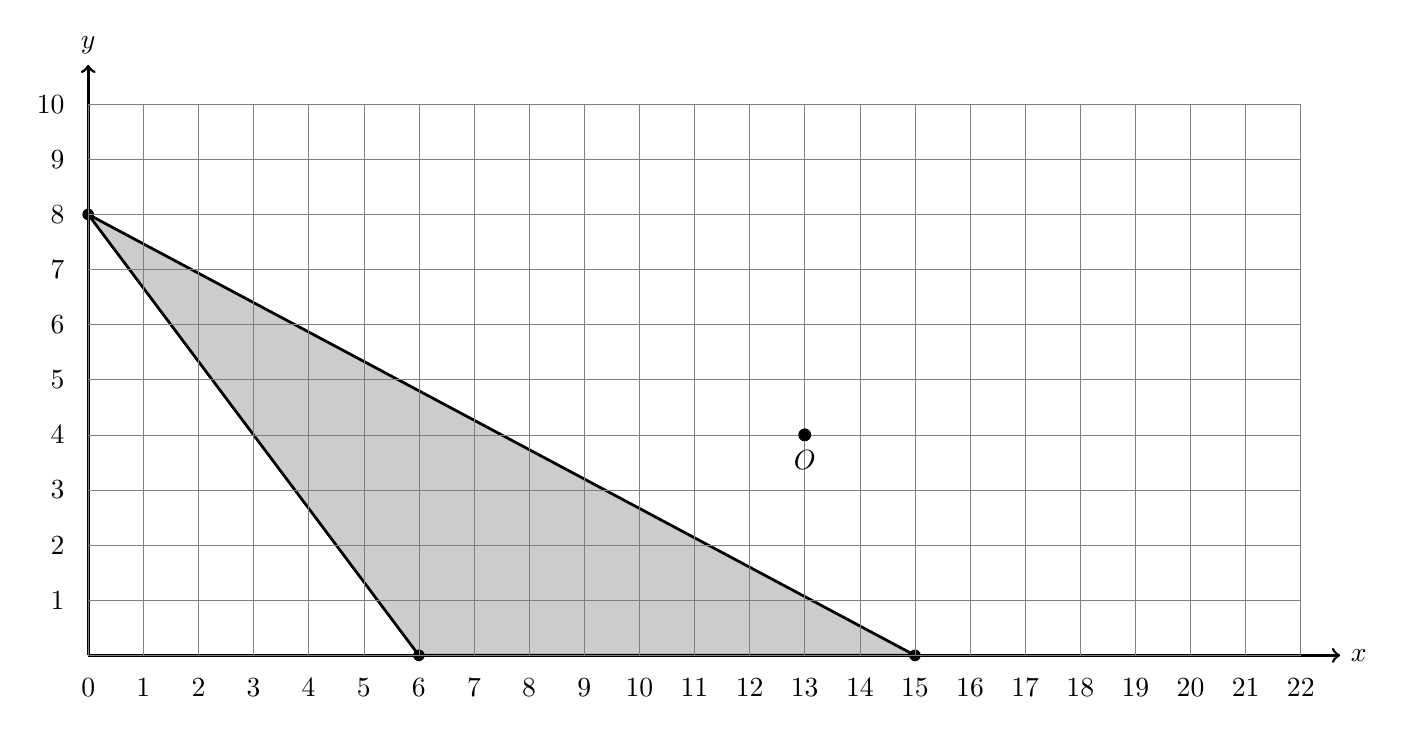
\begin{tikzpicture}[scale=0.7]
        \draw[->,shorten >=-5mm,line width=1pt] (0,0) -- (0,10) node[pos=1,above,yshift=5mm] {$y$};
        \draw[->,shorten >=-5mm,line width=1pt] (0,0) -- (22,0) node[pos=1,right,xshift=5mm] {$x$};
        \foreach \x in {0,...,22} {
            \node[below=5pt] at (\x,0) {$\x$};
        }
        \foreach \y in {1,...,10} {
            \node[left=5pt] at (0,\y) {$\y$};
        }
        \draw[line width=1pt,fill=black!20] (0,8) -- (6,0) -- (15,0) -- (0,8);
        \fill (0,8) circle (3pt);
        \fill (6,0) circle (3pt);
        \fill (15,0) circle (3pt);
        \draw[help lines] (0,0) grid (22,10);
        \node [label=below:$O$,draw,fill=black,circle,inner sep=1.5pt] at (13,4) {}; 
    \end{tikzpicture}
\end{center}

\begin{desarrollo}[height=9cm]
\end{desarrollo}
\begin{respuesta}[height=2cm]
\end{respuesta}

\subsection{} Determine el valor de los segmentos $\overline{AB}$ [2 puntos] y $\overline{AC}$ 
[2 puntos] en la figura a continuación, y justifique en el proceso por qué los segmentos 
$\overline{AB}$ y $\overline{DE}$ son paralelos [1 punto]. 

\begin{center}
\begin{tikzpicture}[ampersand replacement=\&,line width=1pt]
    \draw (0,0) coordinate [label={[label distance=2pt]left:$A$}] (A) -- (-50:4) %
    coordinate [label={[label distance=2pt]below:$B$}] (B) -- ([turn]60:7) %
    coordinate [label={[label distance=2pt]right:$C$}] (C) -- cycle;
    \draw ($(C)!0.4!(A)$) coordinate [label={[label distance=10pt]above:$D$}] (D) %
    -- ($(C)!0.4!(B)$) coordinate [label={[label distance=2pt]below:$E$}] (E);
    \draw pic ["$120$",draw,<->,angle eccentricity=0.5,angle radius=0.7cm] {angle = C--B--A};
    \draw pic ["$120$",draw,<->,angle eccentricity=0.5,angle radius=0.7cm] {angle = C--E--D};
    \draw[decorate, decoration={calligraphic brace,mirror,raise=4pt,amplitude=10pt}]
    (C) -- (D) node [pos=0.5,above=15pt,xshift=3pt] {$8$};
    \draw[decorate, decoration={calligraphic brace,mirror,raise=4pt,amplitude=10pt}]
    (D) -- (A) node [pos=0.5,above=15pt,xshift=3pt] {$2x+2$};
    \draw[decorate, decoration={calligraphic brace,raise=4pt,amplitude=10pt,mirror}]
    (D) -- ($(D)!0.90!(E)$) node [pos=0.5,left=13pt,yshift=-10pt] {$15$};
    \draw[decorate, decoration={calligraphic brace,raise=4pt,amplitude=10pt,mirror}]
    (A) -- ($(A)!0.98!(B)$) node [pos=0.5,left=13pt,yshift=-10pt] {$4x+3$};
\end{tikzpicture}
\end{center}

\begin{desarrollo}[height=12cm]
\end{desarrollo}
\begin{respuesta}[height=4cm]
\end{respuesta}

\end{document}